\documentclass[tikz,border=10pt]{standalone}
\usetikzlibrary{arrows.meta, angles, quotes, calc, positioning}

\begin{document}
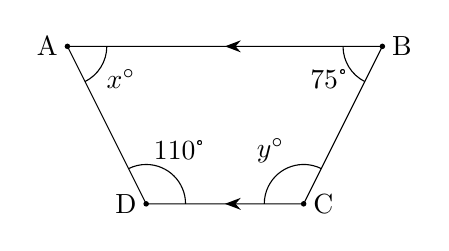
\begin{tikzpicture}
    % Draw trapezoid
    \coordinate (A) at (0,0);
    \coordinate (B) at (4,0);
    \coordinate (C) at (3,-2);
    \coordinate (D) at (1,-2);

    \draw (A) -- (B) -- (C) -- (D) -- cycle;

    % Draw parallel lines indicators
    \draw[thick,{Stealth[length=2mm]}-] ($(D)!0.5!(C)$) -- + (0.1,0);
    \draw[thick,{Stealth[length=2mm]}-] ($(A)!0.5!(B)$) -- + (0.1,0);

    % Label points
    \foreach \point in {A, B, C, D}
        \fill [black,opacity=1] (\point) circle (1pt);

    % Draw angles with adjusted eccentricity and radius
    \pic["110°", draw=black, angle eccentricity=1.6, angle radius=0.5cm] {angle = C--D--A};
    \pic["75°", draw=black, angle eccentricity=1.6, angle radius=0.5cm] {angle = A--B--C};
    \pic["$x^\circ$", draw=black, angle eccentricity=1.6, angle radius=0.5cm] {angle = D--A--B};
    \pic["$y^\circ$", draw=black, angle eccentricity=1.6, angle radius=0.5cm] {angle = B--C--D};

    % Label trapezoid sides
    \draw (A) node[anchor=east] {A};
    \draw (B) node[anchor=west] {B};
    \draw (C) node[anchor=west] {C};
    \draw (D) node[anchor=east] {D};

\end{tikzpicture}
\end{document}